%% Copyright (C) 2019 University of Exeter, UK
%%               2018 The University of Sheffield, UK
%%               2018 The University of Paris-Saclay, France
%%
%% License:
%%   This program can be redistributed and/or modified under the terms
%%   of the LaTeX Project Public License Distributed from CTAN
%%   archives in directory macros/latex/base/lppl.txt; either
%%   version 1 of the License, or any later version.
%%   OR
%%   The 2-clause BSD-style license.
%%  
%%   SPDX-License-Identifier: LPPL-1.0+ OR BSD-2-Clause

%% This is a placeholder for user-specific configuration and packages. 
\usepackage{etex}
\reserveinserts{28}

\usepackage{dirtree}
\renewcommand*\DTstylecomment{\ttfamily\itshape}
\usepackage[scaled=0.88]{beramono}%
\usepackage{upquote}%
\usepackage{textcomp}
\usepackage{xcolor}
\usepackage{paralist}
\usepackage{listings}
\usepackage{lstisadof-manual}
\usepackage{xspace}
\usepackage{dtk-logos}
\usepackage[caption]{subfig}
\usepackage[size=footnotesize]{caption}
\usepackage{railsetup}

\usepackage{index}
\newcommand{\bindex}[1]{\index{#1|textbf}}
%\makeindex
%\AtEndDocument{\printindex}

\newcommand{\ie}{i.e.}
\newcommand{\eg}{e.g.}
\newcommand{\path}[1]{\texttt{\nolinkurl{#1}}}
\title{<TITLE>}
\author{<AUTHOR>}

\newcommand{\dof}{DOF\xspace}
\renewcommand{\listofSRACs}{\relax}
\renewcommand{\listofECs}{\relax}
\pagestyle{headings}

\uppertitleback{
Copyright \copyright{} 2019\phantom{--2019} University of Exeter, UK\\
\phantom{Copyright \copyright{}} 2018--2019 Universit\'e Paris-Saclay, France\\
\phantom{Copyright \copyright{}} 2018--2019 The University of Sheffield, UK\\

\smallskip
\begin{small}
Redistribution and use in source and binary forms, with or without
modification, are permitted provided that the following conditions are
met:
\begin{itemize}
  \item Redistributions of source code must retain the above copyright
        notice, this list of conditions and the following disclaimer.
      \item Redistributions in binary form must reproduce the above
        copyright notice, this list of conditions and the following
        disclaimer in the documentation and/or other materials provided
       with the distribution.
\end{itemize}
\end{small}\begin{small}
THIS SOFTWARE IS PROVIDED BY THE COPYRIGHT HOLDERS AND CONTRIBUTORS ``AS IS''
AND ANY EXPRESS OR IMPLIED WARRANTIES, INCLUDING, BUT NOT LIMITED TO, THE 
IMPLIED WARRANTIES OF MERCHANTABILITY AND FITNESS FOR A PARTICULAR PURPOSE ARE 
DISCLAIMED. IN NO EVENT SHALL THE COPYRIGHT OWNER OR CONTRIBUTORS BE LIABLE 
FOR ANY DIRECT, INDIRECT, INCIDENTAL, SPECIAL, EXEMPLARY, OR CONSEQUENTIAL
DAMAGES (INCLUDING, BUT NOT LIMITED TO, PROCUREMENT OF SUBSTITUTE GOODS OR
SERVICES; LOSS OF USE, DATA, OR PROFITS; OR BUSINESS INTERRUPTION) HOWEVER
CAUSED AND ON ANY THEORY OF LIABILITY, WHETHER IN CONTRACT, STRICT LIABILITY,
OR TORT (INCLUDING NEGLIGENCE OR OTHERWISE) ARISING IN ANY WAY OUT OF THE USE
OF THIS SOFTWARE, EVEN IF ADVISED OF THE POSSIBILITY OF SUCH DAMAGE.
\end{small}

\medskip
\textbf{SPDX-License-Identifier:} BSD-2-Clause
}

\lowertitleback{%
This manual describes \isadof version \isadofversion.  

The latest development version as well as previous releases are available at 
\url{https://git.logicalhacking.com/Isabelle_DOF/Isabelle_DOF}.

\paragraph*{Contributors.} We would like to thank the following contributors to \isadof 
(in alphabetical order): Idir Ait-Sadoune, Paolo Crisafulli, and Chantal Keller.

\paragraph*{Acknowledgments.} This work has been partially supported by IRT SystemX, Paris-Saclay, 
France, and therefore granted with public funds of the Program ``Investissements d'Avenir.''

}



\publishers{
\begin{center}
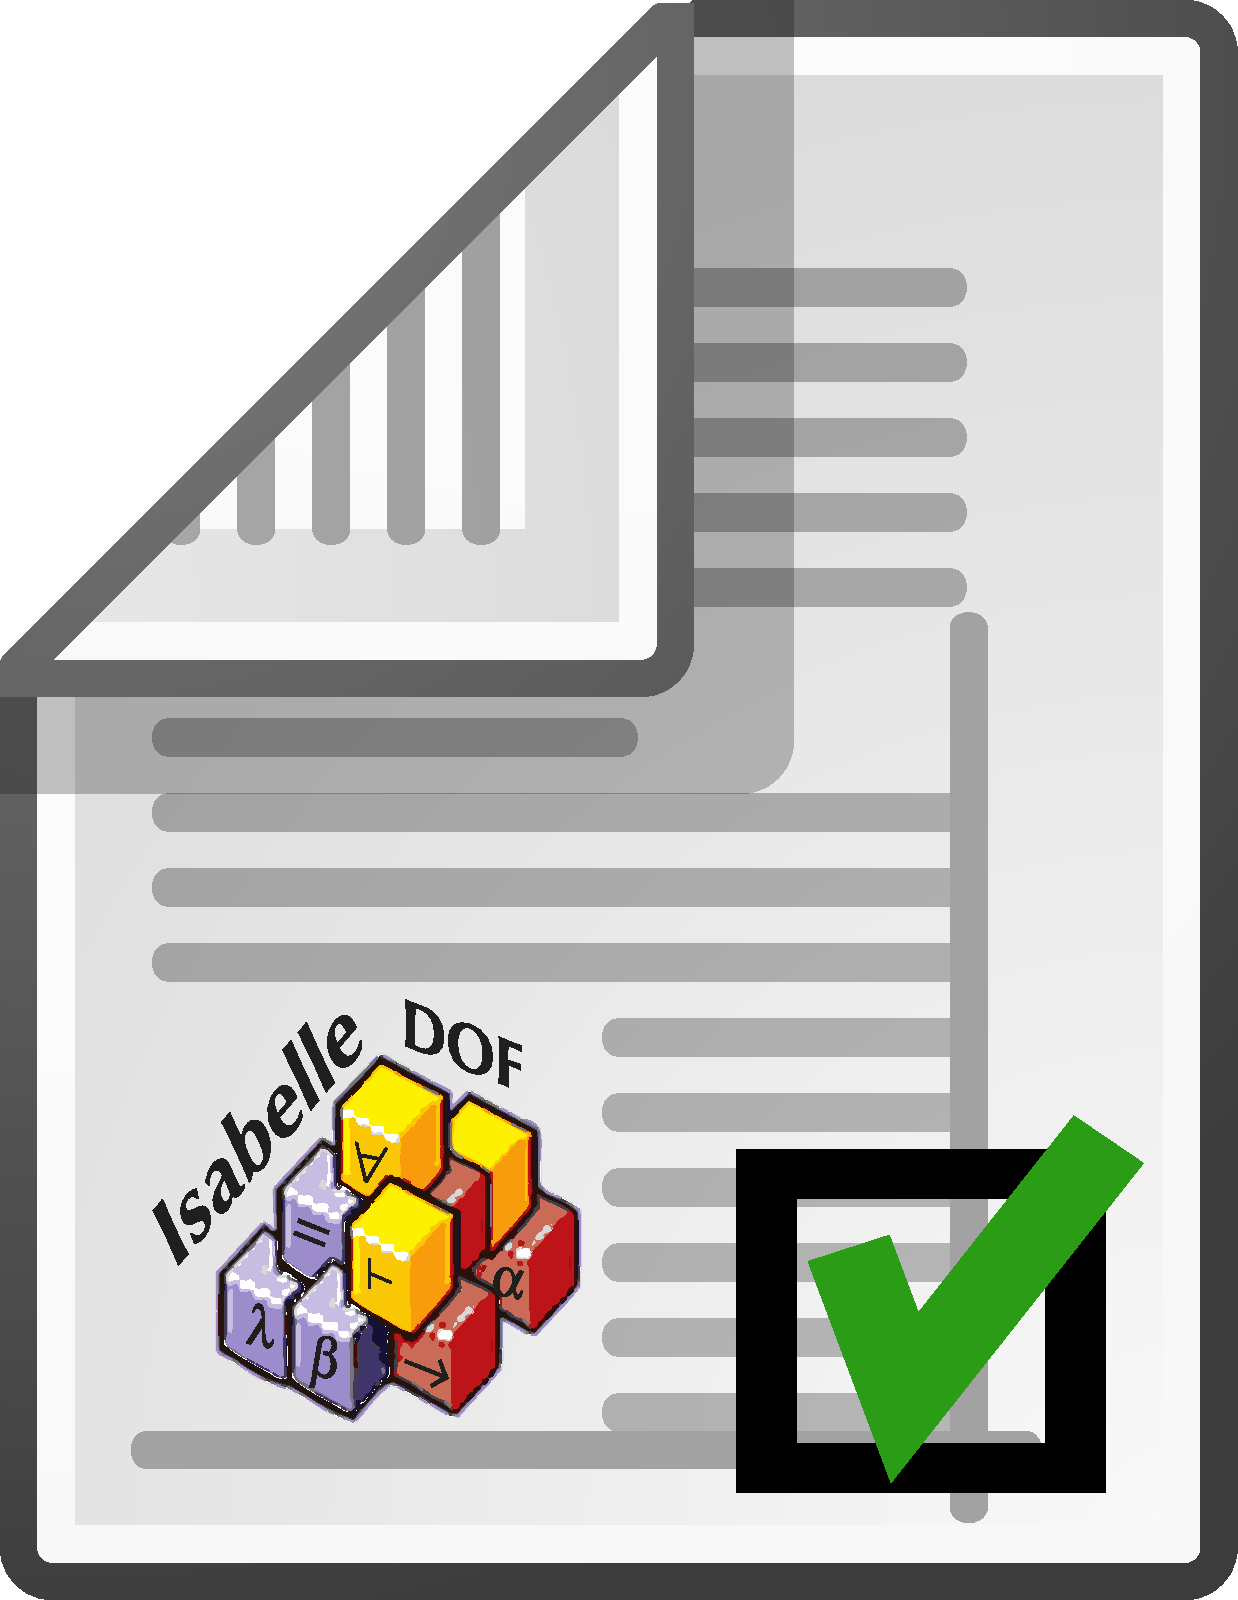
\includegraphics[width=.28\textwidth]{figures/Isabelle_DOF-logo}
\end{center}
\vspace{3cm}

\begin{minipage}{\textwidth}
  \begin{minipage}{6cm}
    \normalsize
    Department of Computer Science\\
    University of Exeter\\
    Exeter, EX4 4QF\\
    UK
  \end{minipage}
  \hfill
  \begin{minipage}{8cm}
    \raggedleft\normalsize
    Laboratoire en Recherche en Informatique (LRI)\\
    Universit\'e Paris-Saclay\\
    91405 Orsay Cedex\\
    France
  \end{minipage}
\end{minipage}
}

\renewcommand{\isacommand}[1]{\textcolor{OliveGreen!60}{\ttfamily\bfseries #1}}
